\documentclass[a4paper]{article}

\usepackage[a4paper]{geometry}

\usepackage[dutch]{babel}

\usepackage{titling}
\pretitle{\begin{center}\LARGE\sffamily\bfseries}
\posttitle{\end{center}}

\predate{\begin{center}\sffamily\bfseries}
\postdate{\end{center}}

\usepackage{sectsty}
\allsectionsfont{\normalfont\sffamily\bfseries}

\usepackage{hyperref}

\usepackage{courier}
\usepackage{color}
\definecolor{consolegray}{gray}{0.9}
\usepackage{listings}

\usepackage[parfill]{parskip}

\usepackage{graphicx}
\usepackage{subfig}

\title{Hands on met de Raspberry Pi}

\begin{document}
  \maketitle
  \tableofcontents

  \section{Inleiding}

  In dit document wordt eerst beschreven hoe je de Raspberry Pi moet
verbinden met de verschillende randapparatuur, hoe je de Raspberry
Pi aanzet, en hoe je de Raspberry Pi de eerste keer configureert.
Daarna wordt beschreven hoe je met de camera en de afstandssensor aan
de slag kan.

    \subsection{Benodigdheden}

    De volgende items zouden zeker in je kit moeten zitten:

    \begin{enumerate}
      \item Raspberry Pi Model A
      \item HDMI naar DVI kabel
      \item SD kaart
      \item Muis \& toetsenbord
      \item USB Hub
      \item USB WiFi dongle
      \item Raspberry Pi camera
      \item Micro USB adapter
    \end{enumerate}

  \section{De Raspberry Pi opstarten}

    Dit hoofdstuk beschrijft hoe je de Raspberry Pi moet aansluiten op
alle randapparatuur.  Daarna zal de Raspberry Pi opstarten.  Indien
het de eerste keer is dat je Raspbian opstart moeten er een aantal
zaken geconfigureerd worden.

    \subsection{De Raspberry Pi connecteren}

      Voor je de Raspberry Pi voor het eerst opstart moet je het
toestel connecteren met alle randapparatuur.  De Raspberry Pi heeft
geen aan/uit knop.  De Pi zal opstarten zodra er stroom is.

      \paragraph{SD kaart} Het slot voor de SD kaart zit onderaan de
Raspberry Pi.  Schuif de SD kaart met de contactpunten naar boven in
het slot.

      \paragraph{Monitor} Kies bij voorkeur een monitor met een vrije
DVI ingang.  Op die manier hoef je geen kabels uit te trekken.  Kies
de DVI ingang als \emph{source} voor de monitor.

      \paragraph{USB toestellen} Sluit de USB hub aan op de USB poort
van de Raspberry Pi.  Je gebruikt hiervoor de stekker waaruit twee
draden vertrekken.  De Wifi dongle, het toetsenbord en de muis sluit
je aan op de USB Hub.

      \paragraph{Micro USB adapter} Connecteer de Micro USB adapter
met de Raspberry Pi.  De Raspberry Pi zal nu opstarten.  Je ziet een
gekleurd vierkant op het scherm verschijnen gevolgd door de Linux boot
sequentie.

    \subsection{Initi\"ele configuratie}

      Wanneer je Raspbian voor het eerst opstart kom je na de start up
in de \texttt{raspi-config} configuratie tool.  Met deze tool kan je
een aantal Raspberry Pi specifieke configuratie instellingen wijzigen.

      Als Raspbian reeds is opgestart van op deze SD kaart zal
\texttt{raspi-config} niet geladen worden en zal je in de plaats
daarvan het login scherm zien.  Normaal gezien zijn alle instellingen
reeds in orde gebracht. 

      Als je de \texttt{raspi-config} tool per ongeluk verlaat kan je
deze terug starten door het volgende commando in de console te typen:

\lstset{emph={pi@raspberrypi,~,$},emphstyle={\textbf},basicstyle={\ttfamily},backgroundcolor=\color{consolegray},framesep=4pt,framexleftmargin=6pt,frame=tb,framerule=0pt}
\begin{lstlisting}
pi@raspberrypi ~ $ sudo raspi-config
\end{lstlisting}

      \paragraph{Filesystem uitbreiden}
      Wanneer de Raspbian software op de SD kaart wordt gezet neemt
deze niet de ganse SD kaart in beslag.  Om meer plaats te hebben in je
filesystem kan je het uitbreiden.

      \begin{enumerate}
        \item Kies optie \texttt{1 Expand Filesystem}.
        \item Even later verschijnt normaal de bevestiging dat de root partitie
groter is gemaakt.  
        \item Druk op \emph{enter}.
      \end{enumerate}

      \paragraph{Correcte toetsenbord layout kiezen}
      De standaard instellingen voor de toetsenbord indeling komt niet
overeen met het toetsenbord dat jullie gekregen hebben.  Je moet het
juiste toetsenbord selecteren door je instelling steeds verder te
verfijnen.

      \begin{enumerate}
        \item Kies optie \texttt{4 Internationalisation Options}.
        \item Kies vervolgens \texttt{I3 Change Keyboard Layout}.
        \item Selecteer \texttt{Generic 105-key (Intl) PC} in de lijst met modellen.
        \item Selecteer \texttt{Other} in de lijst met keyboard layouts.
        \item Selecteer \texttt{English (US)}.
        \item Selecteer \texttt{English (US)} (helemaal bovenaan).
        \item Selecteer \texttt{The default for the keyboard layout}.
        \item Selecteer \texttt{No compose key}
        \item Selecteer \texttt{<Yes>} om via
\texttt{Control+Alt+Backspace} de X server te kunnen stoppen.
      \end{enumerate}

      De nieuwe instellingen zijn onmiddelijk van kracht.

      \paragraph{Camera activeren}
      Om later de camera te kunnen gebruiken moet deze eerst
geconfigureerd worden.  Deze wijziging zal pas actief zijn na een
reboot.

      \begin{enumerate}
        \item Kies optie \texttt{5 Enable Camera}.
        \item In de volgende dialoog kies je voor \texttt{<Enable>}.
      \end{enumerate}

      \paragraph{SSH activeren}
      Op termijn is het eenvoudiger om op de Raspberry Pi in te loggen
via SSH.  Op die manier kan je van op je eigen computer werken en
kunnen meerdere gebruikers tegelijk de Raspberry Pi gebruiken.

      \begin{enumerate}
        \item Kies \texttt{8 Advance Options}.
        \item Kies \texttt{A4 SSH}.
        \item Kies \texttt{<Enable>}.
        \item Je krijgt de bevestiging dat de SSH server vanaf nu
geactiveerd is.
      \end{enumerate}

      \paragraph{Rebooten}  Nadat je de nodige configuratie
instellingen hebt aangepast kan je best je Raspberry Pi rebooten.
Selecteer \texttt{<Finish>} om \texttt{raspi-config} te be\"eindigen.
Kies nadien voor \texttt{<Yes>} om te rebooten.

    \subsection{Inloggen}

      De Raspbian distributie komt met een standaard gebruiker:
\texttt{pi} en paswoord \texttt{raspberry}.  Na het inloggen kom je in
de standaard Linux console.  Je kan de grafische gebruikers interface
starten met:

\begin{lstlisting}
pi@raspberrypi ~ $ startx
\end{lstlisting}

    \subsection{WiFi configureren}

      Om je WiFi connectie te configureren kan je een grafische
configuratie tool gebruiken (\texttt{wpa\_gui}).  De snelkoppeling op je bureaublad werkt
echter niet.  De tool heeft \texttt{root} rechten nodig.

      Open \emph{LXTerminal} via de snelkoppeling op je bureaublad.  Je
krijgt een console te zien.  Je kan de configuratie tool als
\texttt{root} starten met het volgende commando:

\begin{lstlisting}
pi@raspberrypi ~ $ sudo wpa_gui
\end{lstlisting}

    In het venster dat opent klik je op de \emph{Scan} knop onderaan.
Er opent zich een nieuw venster \emph{Scan results}.  Hier moet je
weer op de knop \emph{Scan} drukken om te scannen naar beschikbare
WiFi netwerken.

    Kies het \emph{eduroam} netwerk in de lijst door er op te
dubbelklikken.  Dit opent een configuratie venster voor het
\emph{eduroam} network.

    Op de KULeuven ICTS pagina
\url{https://admin.kuleuven.be/icts/english/wifi/eduroam-ubuntu} vind
je hoe je het eduroam netwerk kan instellen op een Ubuntu Linux.  Het
merendeel van de instellingen is identiek op Raspbian.
Table~\ref{table:eduroam} geeft een overzicht van de configuratie
nodig voor eduroam.

  \begin{table}[h!]
    \centering
    \begin{tabular}{ll}
      \hline
      SSID & eduroam \\
      Authentication & WPA2-Enterprise (EAP) \\
      Encryption & CCMP \\
      EAP method & PEAP \\
      Identity & xxxxxxxxx@kuleuven.be \\
      Password & your-password \\
      CA certificat & \emph{blanco laten} \\
      \hline
    \end{tabular}
    \caption{Configuratie voor het eduroam netwerk in
\texttt{wpa\_gui}.  Het \emph{CA certificat} veld mag blanco blijven.}
    \label{table:eduroam}
  \end{table}

  \section{Opdrachten}

    Dit hoofdstuk beschrijft een aantal opdrachten die je helpen
vertrouwd te worden met de camera en de afstandssensor.

  \subsection{De Raspberry Pi Camera module}

    Je kan foto's en video's nemen met de Raspberry Pi camera module
met behulp van respectievelijk het \texttt{raspistill} en
\texttt{raspivid} commando.

    \subsubsection{De camera module connecteren}
  
    De kabel komende van de camera module moet verbonden worden met de
connector vlak naast de HDMI aansluiting.  De kant met het blauwe
kleeflint moet \emph{weg} wijzen van HDMI connector.  De kant met de metalen
connectors moet \emph{naar} de HDMI connector wijzen
(Figuur~\ref{fig:camera}).

\begin{figure}[h!]
\centering
\subfloat{
  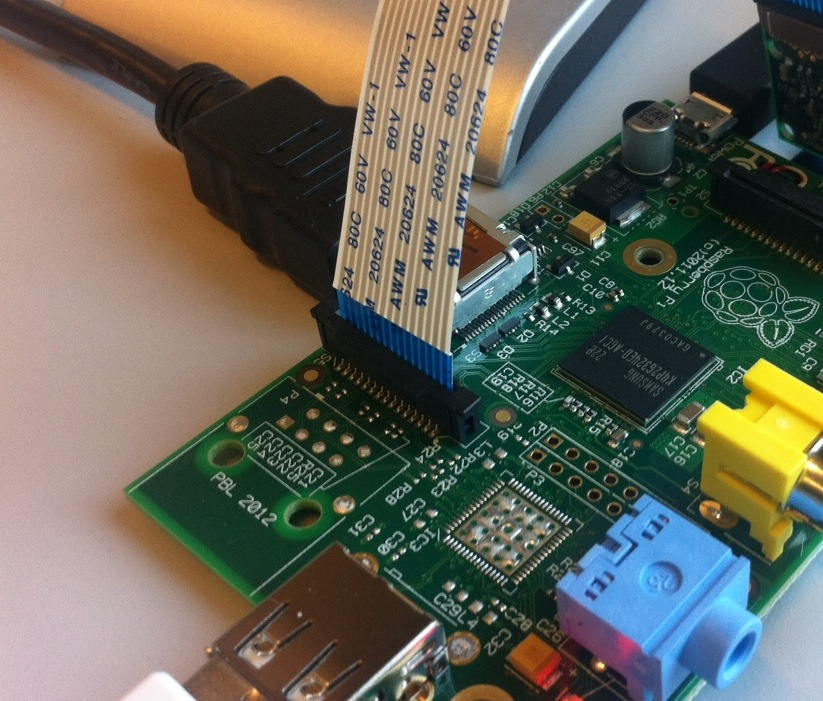
\includegraphics[width=.48\textwidth]{images/camera-2.jpg}
}
\subfloat{
  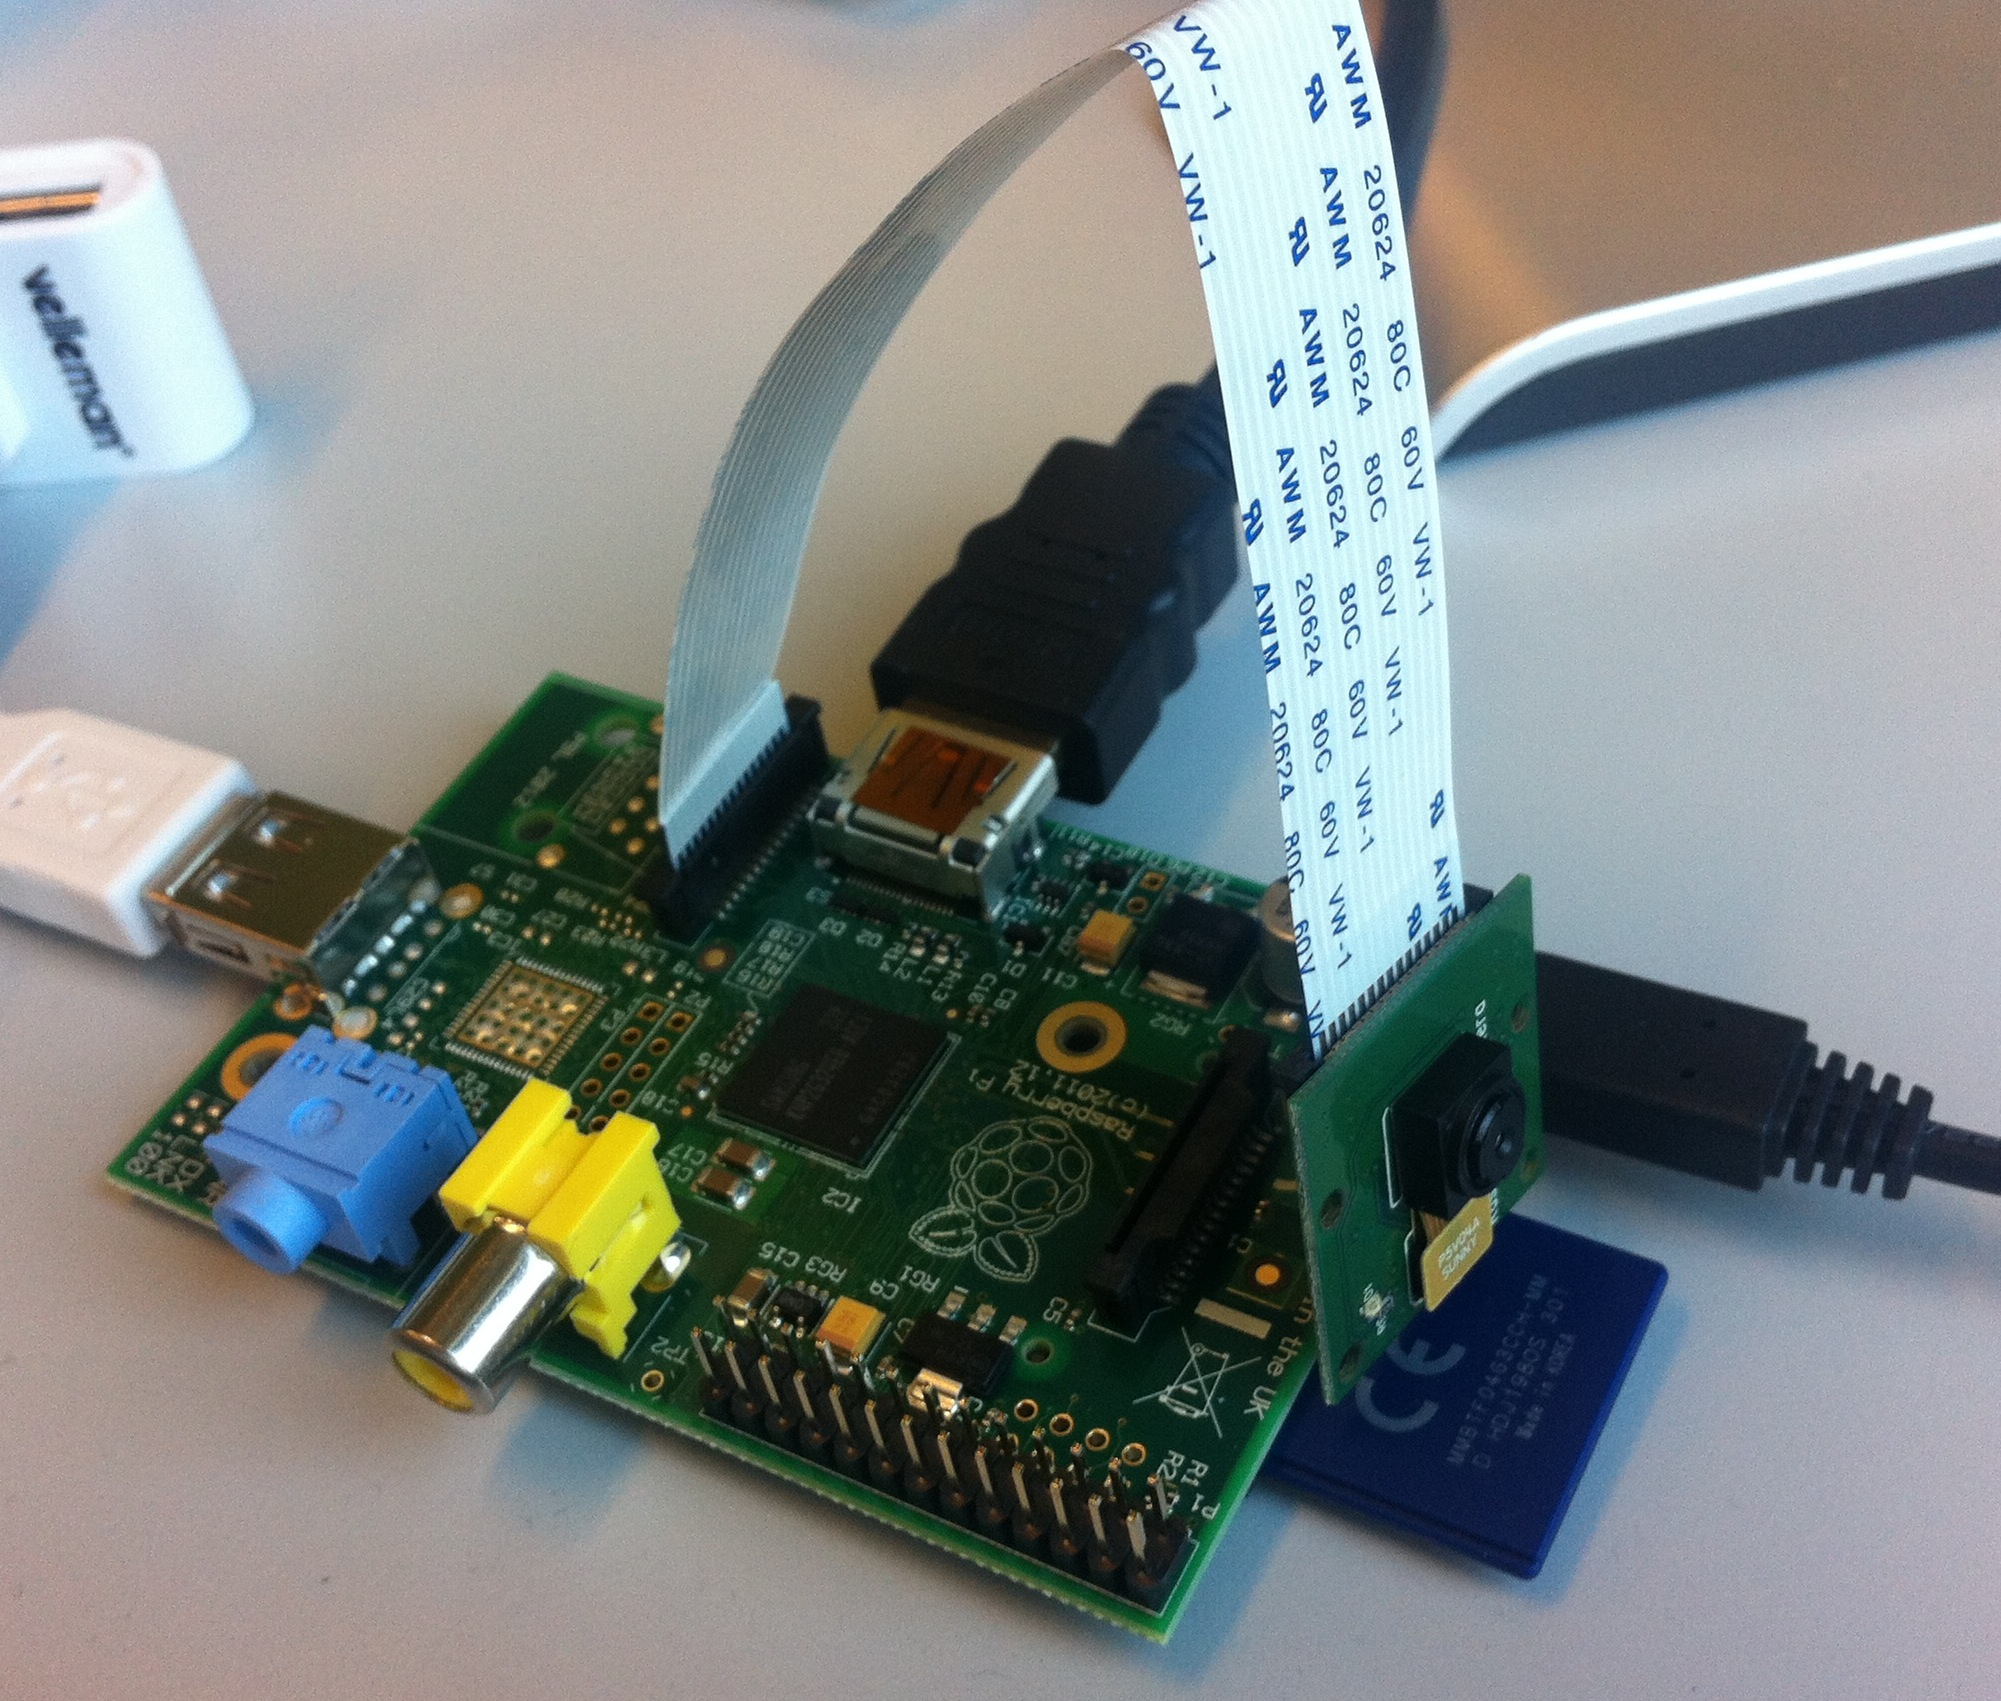
\includegraphics[width=.48\textwidth]{images/camera-1.jpg}
}
\caption{De kant met het blauwe kleeflint moet \emph{weg} wijzen van
HDMI connector.  De kant met de metalen connectors moet \emph{naar} de
HDMI connector wijzen.}
\label{fig:camera}
\end{figure}

    Nadat je de camera hebt aangesloten moet je de Raspberry Pi
herstarten.  Dit kan je doen door in een console het volgende commando
te geven:

\begin{lstlisting}
pi@raspberrypi ~ $ sudo reboot
\end{lstlisting}

    Dit roept het \texttt{reboot} commando aan als \texttt{root}
gebruiker.

    Wanneer de Raspberry Pi opnieuw is opgestart moet je opnieuw
inloggen en de grafische omgeving starten met \texttt{startx}.

    \subsubsection{Foto's nemen met de camera module}

      Met het commandline programma \texttt{raspistill} kan je foto's
nemen.

\begin{lstlisting}
pi@raspberrypi ~ $ raspistill -o image.jpg
\end{lstlisting}

    Na het geven van dit commando komt er op het scherm een preview van
de foto.  Na 5 seconden preview wordt er een foto genomen en bewaard
in de \texttt{image.jpg} file in je huidige directory.

    Je kan de foto nu bekijken met het volgende commando:
\begin{lstlisting}
pi@raspberrypi ~ $ gpicview image.jpg
\end{lstlisting}
    of door in een file browser naar het foto bestand te navigeren en
het zo te openen.

    Het \texttt{raspistill} commando heeft erg veel opties.  Een
overzicht van alle opties krijg je door het volgende commando uit te
voeren.
\begin{lstlisting}
pi@raspberrypi ~ $ raspistill --help
\end{lstlisting}

    \subsubsection{Video's maken met de camera module}

      Met het commandline programma \texttt{raspivid} kan je video's
opnemen. Het volgende commando maakt een video van 10 seconden en
schrijft deze video weg in het \texttt{video.h264} bestand.
\begin{lstlisting}
pi@raspberrypi ~ $ raspivid -o video.h264 -t 10000
\end{lstlisting}

      Je kan de video bekijken met de \texttt{omxplayer} player:
\begin{lstlisting}
pi@raspberrypi ~ $ omxplayer video.h264
\end{lstlisting}

      Net als \texttt{raspistill} heeft \texttt{raspivid} veel
configuratie opties.  Je krijg een overzicht van al deze opties met
het commando:
\begin{lstlisting}
pi@raspberrypi ~ $ raspivid --help
\end{lstlisting}

  \subsection{De afstandssensor}

    In dit deel wordt beschreven hoe je waarden van de afstandssensor
uitleest met behulp van Python of Java.  Om te werken met de
afstandssensor moet je gebruik maken van de GPIO pinnen.

    \subsubsection{Werking van de GPIO pinnen}

      De Raspberry Pi heeft in totaal 26 GPIO pinnen.  Hiervan kunnen
er 17 gebruikt worden voor algemene in- en uitvoer.
Figuur~\ref{fig:gpio} toont de verschillende pinnen.

      \begin{figure}[h!]
        \centering
        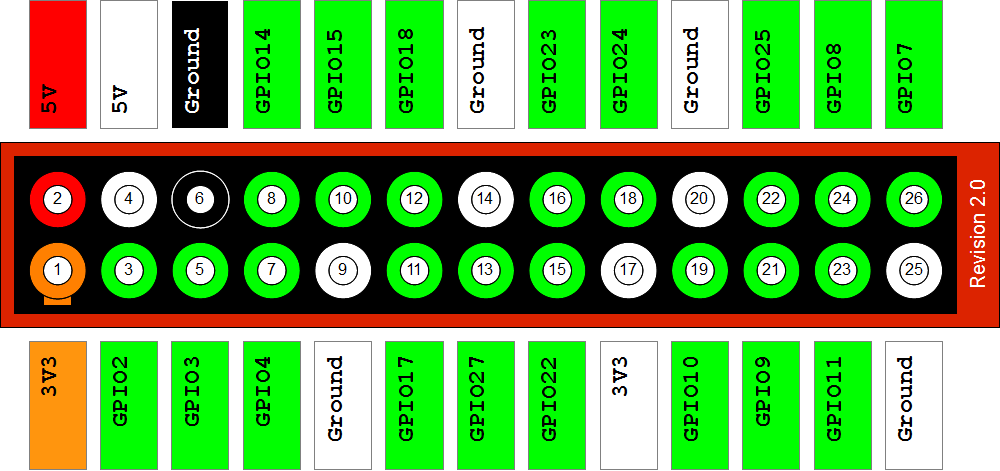
\includegraphics[width=.8\textwidth]{images/gpio.png}
        \caption{De verschillende GPIO pinnen.  De pinnen worden op
twee verschillende manieren benoemd: op basis van hun fysieke locatie
(nummer in de cirkels) of op basis van hun connectie met de CPU (de
GPIOXX labels in het groen).}
        \label{fig:gpio}
      \end{figure}

      Pin 1, links onderaan Figuur~\ref{fig:gpio}, heeft onderaan een
rechthoekig symbool. Pin 1 op de Raspberry Pi heeft hetzelfde symbool.

      De pinnen kunnen op twee manieren benoemd worden.  Op basis van
de fysieke locatie van de pin en op basis van de connectie met de CPU.
De fysieke locatie wordt als volgt bepaald: De pin met symbool, 
onderaan links is pin 1. De pin daarboven is pin 2.  De pin rechts van
pin 1 is pin 3.  De pin boven pin 3 is pin 4.  En zo verder.  De
fysieke pin nummers worden getoond in Figuur~\ref{fig:gpio:physical}.

      \begin{figure}[h!]
        \centering
        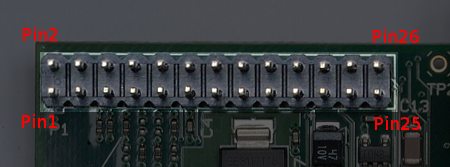
\includegraphics[width=.8\textwidth]{images/gpio-physical.png}
        \caption{De fysieke pin nummering}
        \label{fig:gpio:physical}
      \end{figure}

      De alternatieve benaming voor de pinnen is gebaseerd op hun
connectie met de CPU.  Zo is de pin op plaats 3 verbonden met ingang 2
van de CPU, en de pin op plaats 5 is verbonden met ingang 3 van de
CPU.  Deze pinnen krijgen dus respectievelijk de labels \texttt{GPIO2}
en \texttt{GPIO3}.

      Figuur~\ref{fig:gpio} toont de mapping tussen beide benamingen.
Enkel de pinnen met een groen label zijn verbonden met de CPU en
hebben een \texttt{GPIO} label.  Enkel deze pinnen kunnen gebruikt
worden voor in en uitvoer.

      De GPIO pinnen kunnen werken in twee verschillende modi.  Ze
werken als invoer of als uitvoer.  Van een pin in invoer modus kan je
in je software lezen of er spanning ten opzichte van de aarding op
staat.  Op een pin in uitvoer modus kan je een spanning ten opzichte
van de aarding plaatsen.

      De GPIO pinnen, de groene pinnen in Figuur~\ref{fig:gpio}, mogen
niet gebruikt worden om stroom te leveren.  Ze dienen enkel maar om
een signaal te geven.  Omwille van hun rechtstreekse verbinding met de
CPU kan een te grote stroom doorheen deze pinnen leiden tot schade aan
de CPU.

      De overige pinnen, de \texttt{3V3}, \texttt{5V} en
\texttt{Ground} pinnen mogen wel gebruikt worden om stroom aan
sensoren te leveren.  Ze kunnen echter enkel de door de Raspberry Pi
ongebruikte stroom leveren.  Als de Micro USB adapter 500 mA levert en
de Raspberry Pi 300 mA verbruikt kunnen de pinnen samen maar 200 mA
leveren.  Voor sensoren zoals de afstandssensor is dit voldoende, voor
het aansturen van een motor is dit wellicht niet voldoende.

    \subsubsection{Werking van de afstandssensor}

      De HC SR04 afstandssensor heeft 4 pinnen, gelabeled \emph{Vcc},
\emph{Trig}, \emph{Echo} en \emph{Gnd}.  De buitenste twee, \emph{Vcc}
en \emph{Gnd}, dienen om de sensor van stroom te voorzien.  De
binnenste twee, \emph{Trig} en \emph{Echo}, dienen respectievelijk om
de sensor te activeren en uit te lezen.

      Wanneer via een GPIO pin in uitvoer modus een signaal gegeven
wordt aan de \emph{Trig} pin zal de sensor een korte ultrasone puls
verzenden.  Nadien zal de sensor een spanning plaatsen op de
\emph{Echo} pin.  Deze spanning kan gedetecteerd worden met een GPIO
pin in invoer modus.  De duur van de spanning komt overeen met de tijd
die het signaal nodig had om het dichtstbijzijnde object te bereiken,
te weerkaatsen en terug te keren naar
sensor\footnote{url: \url{http://elecfreaks.com/store/download/HC-SR04.pdf}}.
Door de lengte van het signaal te meten ($\Delta t$) kan je dus de afstand tot het
object berekenen ($d$) met de formule:

    \begin{equation}
      d = \frac{\Delta t * v_{snd}}{2}
    \end{equation}

      De snelheid van het geluid, $v_{snd}$ in de formule, is 340 m/s.
Om de afstand in centimeters te bereken op basis van een tijdsduur in
microseconden ($\mu s$) volstaat het dus $\Delta t$ te
vermenigvuldigen met $0.017$.

    \subsubsection{Connecteren van de afstandssensor}

      Connecteer de \emph{Vcc} pin van de sensor met pin 2
(\texttt{5V}) van de
Raspberry Pi.  Connecteer de \emph{Gnd} pin van de sensor met pin 25
(\texttt{Ground}) van de Raspberry Pi.  Connecteer de \emph{Trig} pin van de
sensor met pin 7 (\texttt{GPIO4}) van de Raspberry Pi.  En connecteer tot
slot de \emph{Echo} pin van de sensor met pin 11 (\texttt{GPIO17}).
De uiteindelijke connecties moeten overeen komen met
Figuur~\ref{fig:sensor}.

\begin{figure}[h!]
  \centering
\subfloat{
  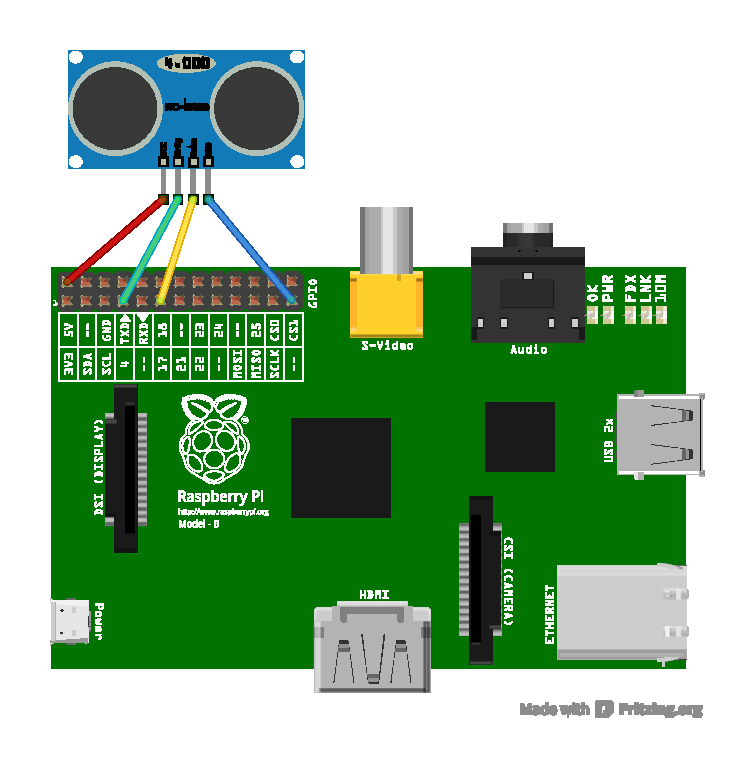
\includegraphics[width=.48\textwidth]{images/sensor.pdf}
}
\subfloat{
  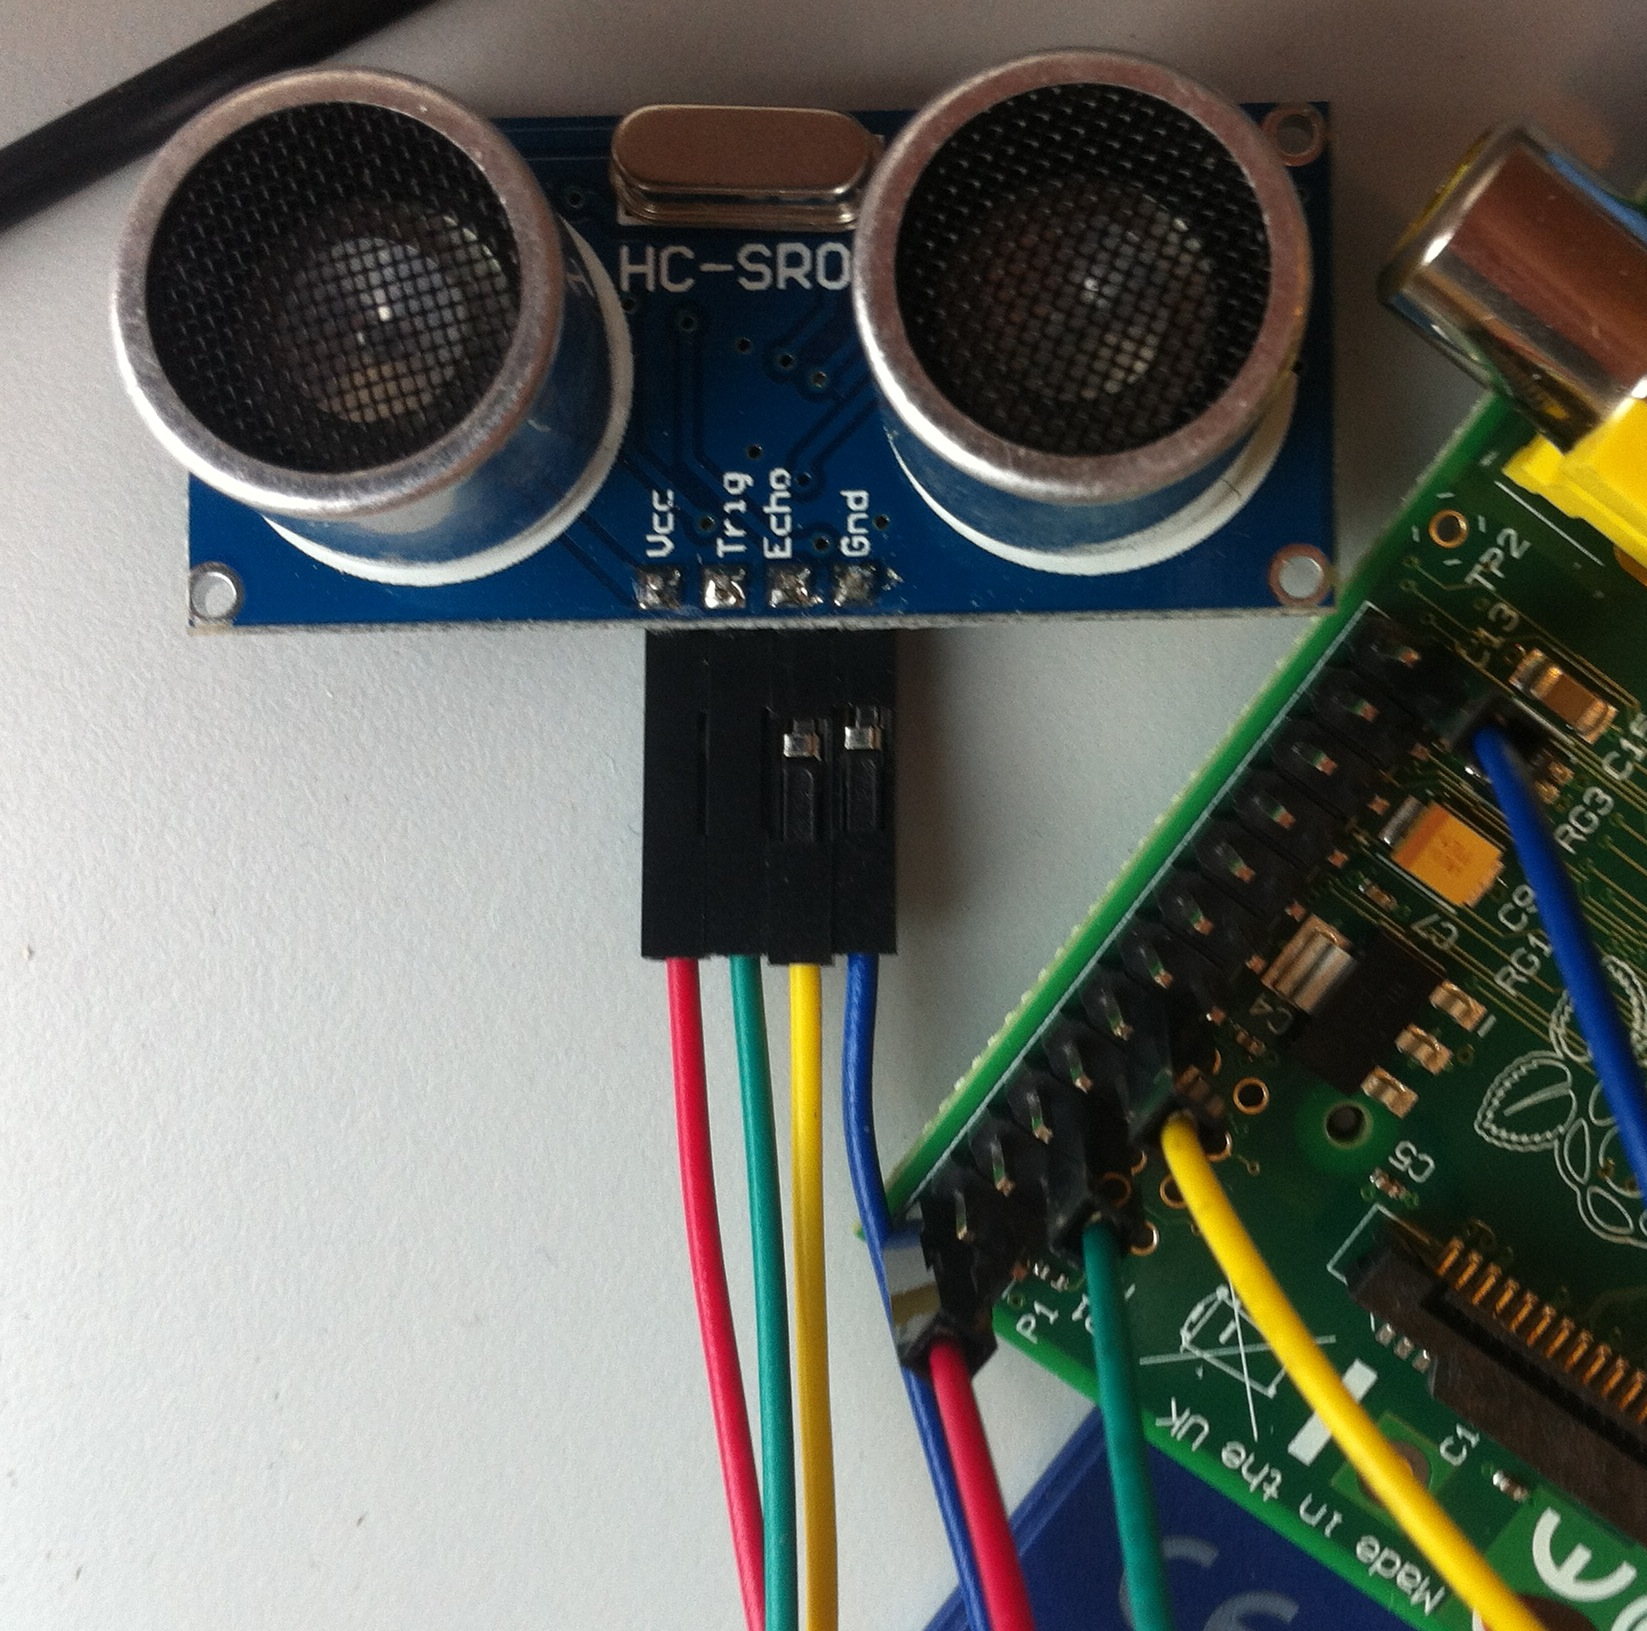
\includegraphics[width=.48\textwidth]{images/sensor.jpg}
}
\caption{De verbinding tussen de afstandssensor en de Raspberry Pi}
\label{fig:sensor}
\end{figure}
  
    \subsubsection{Sensor waarden uitlezen met Python}

    Listing~\ref{lst:distance.py} toont de code nodig om de
afstandssensor uit te lezen op de Pi.  Je kan deze code ook op het
internet bekijken op \url{https://gist.github.com/rutgerclaes/6701244}.  
Om de code snel op de Pi te krijgen kan je volgend command gebruiken:

\begin{lstlisting}
pi@raspberrypi ~ $ wget -O distance.py http://goo.gl/X9ot8j
\end{lstlisting}

\lstinputlisting[language=Python,basicstyle={\footnotesize\ttfamily},label={lst:distance.py},caption={distance.py}]{code/distance.py}

  Je kan het \texttt{distance.py} programma aanpassen met een editor
zoals \texttt{leafpad}.  Nadien moet je het script uitvoerbaar maken
en uitvoeren als \texttt{root}.

\begin{lstlisting}
pi@raspberrypi ~ $ chmod +x distance.py
pi@raspberrypi ~ $ sudo ./distance.py
\end{lstlisting}

  Van zodra het programma gestart is zie je de afstandswaarden voorbij
komen.  Je kan het programma afsluiten met \texttt{Ctrl+c}.

    \subsubsection{Sensor waarden uitlezen met Java}

\end{document}

% vim: tw=70 nocindent expandtab
